\Variant{12.10.2024 (1-smena)}
\QQ{1}{$2321$ sonining $2$ ta tub böluvçisi bor. Şularning yiğindisini toping.
\Opts{$221$}{$211$}{$222$}{$200$}}
\QQ{2}{$2022^{2026}$ sonni $5$ ga bölgandagi qoldiq bilan $2027^{2025}$ sonning oxirgi raqamiga köpaytmasini toping.
\Opts{$14$}{$28$}{$20$}{$24$}}
\QQ{3}{$3$ ta bir xil stulning narxi bitta stol narxining $90\%$iga teng bölsa, $4$ ta huddi şunday stulning narxi bitta stol narxining neça foizini taşkil qiladi?
\Opts{$120$}{$130$}{$125$}{$110$}}
\QQ{4}{$1$ ar yerni Sardor $80$ soatda, Sardor va Bobur $1$ ar yerni $60$ soatda, Sardor va Abror $1$ ar yerni $40$ soatda haydasa, uççalasi birgalikda $1$ ar yerni neça soatda haydaydi?
\Opts{$33\dfrac37$}{$33\dfrac27$}{$34\dfrac37$}{$34\dfrac27$}}
\QQ{5}{Soddalaştiring:
\[\frac{x^{\frac35}y^{-2}}{x^{-\frac12}y^{\frac73}}\]
\Opts{$x^{\frac{11}{10}}y^{\frac{13}3}$}{$x^{\frac{11}{10}}y^{-\frac{13}3}$}{$x^{\frac{11}{10}}y^{\frac{11}3}$}{$x^{\frac{11}{10}}y^{-\frac{11}3}$}}
\QQ{6}{Hisoblang:
\[\frac{\left(\sqrt3+1\right)^2}{2+\sqrt3}+\frac{\left(\sqrt7-1\right)^2}{\sqrt7-4}\]
\Opts{$0$}{$4$}{$-4$}{$1$}}
\QQ{7}{Hisoblang:
\[\frac{\sqrt{18-12\sqrt2}}{\sqrt[4]{\left(2-2\sqrt2\right)^4}}\]
\Opts{$\dfrac{\sqrt6}3$}{$-\dfrac{\sqrt6}3$}{$\dfrac{\sqrt6}2$}{$-\dfrac{\sqrt6}2$}}
\QQ{8}{Soddalaştiring:
\[\frac{abc-a^3}{a^2b}+\frac{abc-b^3}{b^2c}+\frac{abc-c^3}{c^2a}\]
\Opts{$\dfrac{2a}b$}{$1$}{$0$}{$-\dfrac ab$}}
\QQ{9}{$30$ bilan $86$ sonlar orasiga $7$ ta son şunday joylaştirildiki, ular berilgan sonlar bilan birga arifmetik progressiyani taşkil qiladi. Qöyilgan sonlar yiğindisini toping.
\Opts{$204$}{$302$}{$406$}{$248$}}
\QQ{10}{Çeksiz kamayuvçi geometrik progressiya uçun $b_1b_2b_3=5832$ va $b_1+b_2+b_3=78$ bölsa, hadlar yiğindisini toping.
\Opts{$54$}{$78$}{$81$}{$108$}}
\QQ{11}{$a+b=3$, $ab=-1$, $c=-1$ bölsa, $\dfrac{a^2(b-c)-b^2(a-c)}{a(b-c)^2-b(a-c)^2}$ ning qiymatini toping.
\Opts{$1$}{$-1$}{$0$}{$-2$}}
\QQ{12}{Tengsizlikni yeçing:
\[\frac{25x-5}{|x-1|}>0\]
\Opts{$\left(\dfrac15;\,\infty\right)$}{$(1;\,\infty)$}{$\left(\dfrac15;\,1\right)\cup(1;\,\infty)$}{$\left(-\infty;\,\dfrac15\right)$}}
\QQ{13}{$7x^2-6x+1=0$ tenglamaning ildizlari $x_1$ va $x_2$ bölsa, ildizlari $\dfrac1{x_1^2}$ va $\dfrac1{x_2^2}$ bölgan keltirilgan kvadrat tenglamaning koeffitsiyentlari yiğindisini toping.
\Opts{$72$}{$28$}{$29$}{$71$}}
\QQ{14}{Tengsizlikning butun yeçimlari yiğindisini toping:
\[\sqrt[4]{(x-2)^4}\cdot\left(x^2-x-12\right)<0\]
\Opts{$0$}{$2$}{$4$}{$1$}}
\QQ{15}{$\tg\alpha=-\dfrac34$ va $\alpha\in\left(\dfrac\pi2;\,\pi\right)$ bölsa, $\sin\alpha$ ning qiymatini toping.
\Opts{$\dfrac34$}{$\dfrac35$}{$\dfrac16$}{$\dfrac45$}}
\QQ{16}{$\sqrt{\log_x\sqrt{4x}}=-\dfrac1{\log_4x}$ tenglamaning haqiqiy ildizlari yiğindisini toping (agar u yagona bölsa, şuni toping).
\Opts{$\dfrac18$}{$\dfrac14$}{$\dfrac1{16}$}{Yeçimga ega emas}}
\QQ{17}{$2^{x+1}+\dfrac{15}{2^x+1}=11$ tenglamaning haqiqiy ildizlari yiğindisini toping.
\Opts{$1$}{$2$}{$3$}{$-2$}}
\QQ{18}{Tenglamaning ildizlari yiğindisini toping.
\[\sqrt[3]{x+4}+\frac4{\sqrt[3]{x+4}+3}=2\]
\Opts{$-12$}{$-15$}{$-8$}{$12$}}
\QQ{19}{$y=\dfrac{\sqrt{-x^2+3x+10}}{\left|1-\log_x2\right|\cdot\left(\sin x-\frac\pi3\right)}$ aniqlaniş sohasiga tegişli butun sonlar neçta?
\Opts{$5$}{$4$}{$3$}{$2$}}
\QQ{20}{Soddalaştiring:
\[\frac{\sin\alpha+\sin2\alpha+\sin3\alpha+\dots+\sin15\alpha}{\cos\alpha+\cos2\alpha+\cos3\alpha+\dots+\cos15\alpha}\]
\Opts{$2\tg16\alpha$}{$\tg16\alpha$}{$2\tg8\alpha$}{$\tg8\alpha$}}
\QQ{21}{Aniqmas integralni toping:
\[\int\frac{\ln\ln x}x\,dx\]
\Opts{$\ln\ln x+C$}{$\ln x(\ln x-1)+C$}{$\ln x(\ln\ln x+1)+C$}{$\ln x(\ln\ln x-1)+C$}}
\QQ{22}{Quyidagi funksiyalardan neçtasi juft funksiya?
\[y_1=\sin^2x+\sqrt[3]{|x|};\quad y_2=\cos^2x+\sqrt[5]{x^4};\quad y_3=\ctg^3x+\sqrt[3]{x^2};\quad y_4=\sin^4x+\sqrt[5]{x^6}\]
\Opts{$1$ ta}{$2$ ta}{$3$ ta}{$4$ ta}}
\QQ{23}{Radiusi $4$ ga teng aylanaga muntazam ön ikkiburçak içki çizilgan. Ön ikkiburçakning yuzini toping.
\Opts{$24$}{$48$}{$64$}{$80$}}
\QQ{24}{$ABCD$ töğri törtburçakning $A$ uçi koordinatalar boşida, $B$ uçi $Ox$ öqida. $C$ uçining koordinatasi $(5;\,4)$ va $\dfrac12\overrightarrow{BE}=\overrightarrow{BC}$ bölsa, $ABED$ törtburçakning yuzini toping.
\Opts{$15$}{$20$}{$30$}{$40$}}
\QQ{25}{Grafikdan foydalanib quyidagi munosabatlardan neçtasi töğri?
\[\text{a) } f'(b)\cdot g(e)>0;\quad \text{b) } f'(c)\cdot g(a)>0;\quad \text{c) } f'(d)\cdot g(c)>0;\quad \text{d) } f'(d)\cdot g(e)>0\]
\qfig{\begin{tikzpicture}[x=0.6cm,y=1.1cm,font=\small]
\draw[-{Stealth[length=4pt]}] (-5.3,0)--(3.8,0) node[right] {$x$}; \draw[-{Stealth[length=4pt]}] (0,-1.6)--(0,1.9) node[left] {$y$};
\draw[thick,domain=-4.85:3.25,samples=80] plot (\x,{0.07*(\x+4.5)*(\x+1.5)*(\x-2.5)}); \node[right] at (3.2,1.6) {$f(x)$};
\draw[thick,domain=-5.2:3.7] plot (\x,{-0.22*\x}); \node[below] at (3.5,-0.85) {$g(x)$};
\draw[dashed] (-3.19,0)--(-3.19,0.88); \draw[dashed] (-2.096,0)--(-2.096,0.461); \draw[dashed] (-1.8,0)--(-1.8,0.244); \draw[dashed] (1.6,0)--(1.6,-0.352);
\node[below] at (-4.6,0) {$a$}; \node[below] at (-3.19,0) {$b$}; \node[below] at (-2.2,0) {$c$}; \node[below] at (-1.7,0) {$d$}; \node[below left] at (0,0) {$O$}; \node[above] at (1.6,0) {$e$};
\end{tikzpicture}}
\Opts{$1$ ta}{$2$ ta}{$3$ ta}{heç biri töğri emas}}
\QQ{26}{$ABC$ va $ADC$ teng yonli uçburçaklar. $AB=BC=20$, $AD=DC=15$ va $AC=24$ bölsa, $BD=x$ ning qiymatini toping.
\qfig{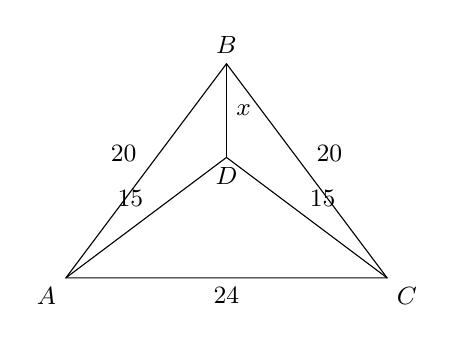
\begin{tikzpicture}[scale=0.17,font=\small]
\coordinate (A) at (-12,0); \coordinate (C) at (12,0); \coordinate (B) at (0,16); \coordinate (D) at (0,9);
\draw (A)--(B)--(C)--cycle; \draw (A)--(D)--(C); \draw (B)--(D);
\node[below left] at (A) {$A$}; \node[below right] at (C) {$C$}; \node[above] at (B) {$B$}; \node[below] at (D) {$D$};
\node[above left] at (-6,8) {$20$}; \node[above right] at (6,8) {$20$}; \node[above left] at (-5.5,4.6) {$15$}; \node[above right] at (5.5,4.6) {$15$}; \node[below] at (0,0) {$24$}; \node[right] at (0,12.5) {$x$};
\end{tikzpicture}}
\Opts{$9$}{$7$}{$8$}{$10$}}
\QQ{27}{$ABCD$, $AMNK$, $MEFL$, $FGNL$ — kvadratlar. Agar $EF=5$ bölsa, $FNC$ uçburçakning yuzini toping.
\qfig{\begin{tikzpicture}[scale=0.13,font=\small]
\coordinate (E) at (0,0); \coordinate (M) at (5,0); \coordinate (A) at (15,0); \coordinate (D) at (35,0); \coordinate (F) at (0,5); \coordinate (L) at (5,5); \coordinate (G) at (0,10); \coordinate (N) at (5,10); \coordinate (K) at (15,10); \coordinate (B) at (15,20); \coordinate (C) at (35,20);
\fill[qfill] (F)--(N)--(C)--cycle;
\draw (E)--(D)--(C)--(B)--(A); \draw (E)--(G)--(N)--(K); \draw (F)--(L); \draw (M)--(N); \draw (F)--(N)--(C)--cycle;
\draw (14.3,5)--(15.7,5); \draw (14.3,15)--(15.7,15);
\node[below] at (E) {$E$}; \node[below] at (M) {$M$}; \node[below] at (A) {$A$}; \node[below] at (D) {$D$}; \node[left] at (F) {$F$}; \node[below right] at (L) {$L$}; \node[left] at (G) {$G$}; \node[above] at (N) {$N$}; \node[below right] at (K) {$K$}; \node[above] at (B) {$B$}; \node[above right] at (C) {$C$};
\node[left] at (0,2.5) {$5$};
\end{tikzpicture}}
\Opts{$50$}{$100$}{$55$}{$40$}}
\QQ{28}{$ABC$ teng yonli uçburçakka içki aylana çizilgan ($AB=AC$). Aylana uçburçakning $AB$ tomonini uriniş nuqtasida $6$ va $4$ ga teng kesmalarga ajratadi. Agar $AB>BC$ bölsa, uçburçakning yuzini toping.
\qfig{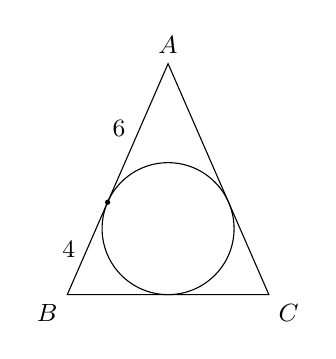
\begin{tikzpicture}[scale=0.32,font=\small]
\coordinate (B) at (-4,0); \coordinate (C) at (4,0); \coordinate (A) at (0,9.165); \coordinate (K) at (-2.4,3.666);
\draw (A)--(B)--(C)--cycle; \draw (0,2.619) circle (2.619); \fill (K) circle (3pt);
\node[above] at (A) {$A$}; \node[below left] at (B) {$B$}; \node[below right] at (C) {$C$};
\node[left] at (-1.3,6.6) {$6$}; \node[left] at (-3.3,1.8) {$4$};
\end{tikzpicture}}
\Opts{$96$}{$48$}{$16\sqrt{21}$}{$8\sqrt{21}$}}
\QQ{29}{$O$ — katta aylana markazi va markazi $B$ va $D$ bölgan aylanalar $O$ nuqtada urinadi. Markazi $C$ va $D$ da bölgan aylanalarning radiuslari mos ravişda $r$ va $R$ bölsa, $\dfrac rR$ ning qiymatini toping.
\qfig{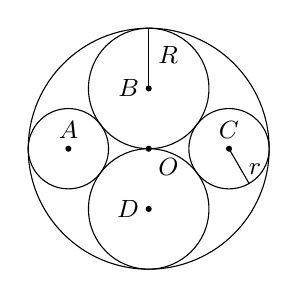
\begin{tikzpicture}[scale=0.85,font=\small]
\draw (0,0) circle (1.8); \draw (0,0.9) circle (0.9); \draw (0,-0.9) circle (0.9); \draw (1.2,0) circle (0.6); \draw (-1.2,0) circle (0.6);
\foreach \p in {(0,0),(0,0.9),(0,-0.9),(1.2,0),(-1.2,0)} \fill \p circle (1.3pt);
\draw (0,0.9)--(0,1.8); \draw (1.2,0)--(1.5,-0.52);
\node[below right] at (0,0) {$O$}; \node[left] at (0,0.9) {$B$}; \node[left] at (0,-0.9) {$D$}; \node[above] at (1.2,0) {$C$}; \node[above] at (-1.2,0) {$A$};
\node[right] at (0,1.4) {$R$}; \node[right] at (1.35,-0.3) {$r$};
\end{tikzpicture}}
\Opts{$\dfrac34$}{$\dfrac45$}{$\dfrac12$}{$\dfrac23$}}
\QQ{30}{$AB$ kesma uçlaridan tekislikkaça bölgan masofalar mos ravişda $AC=12$, $BD=6$ va $\dfrac{BE}{EA}=\dfrac12$ bölsa, $E$ dan tekislikkaça bölgan masofani toping.
\qfig{\begin{tikzpicture}[scale=0.85,font=\small]
\fill[qfill] (1.2,0) ellipse (2.6 and 0.5); \draw (1.2,0) ellipse (2.6 and 0.5);
\coordinate (C) at (0,0); \coordinate (D) at (2.4,0); \coordinate (A) at (0,2); \coordinate (B) at (2.4,1); \coordinate (E) at (1.6,1.333);
\draw (A)--(B); \draw[dashed] (A)--(C); \draw[dashed] (B)--(D); \draw (C)--(D); \fill (E) circle (1.3pt);
\draw (0,0.15)--(0.15,0.15)--(0.15,0); \draw (2.4,0.15)--(2.25,0.15)--(2.25,0);
\node[above] at (A) {$A$}; \node[above right] at (B) {$B$}; \node[above] at (E) {$E$}; \node[below left] at (C) {$C$}; \node[below right] at (D) {$D$};
\node[left] at (0,1) {$12$}; \node[right] at (2.4,0.5) {$6$};
\end{tikzpicture}}
\Opts{$8$}{$9$}{$6$}{$7$}}
\QQ{31}{$A=\{2,\ 3,\ 5,\ 7,\ 9\}$; $B=\{3,\ 4,\ 6,\ 7\}$; $C=\{2,\ 4,\ 7,\ 3,\ 6,\ 11\}$ bölsa, $(A\cap B)\cup C$ ning qism töplamlar sonini toping.
\Opts{$64$}{$128$}{$256$}{$512$}}
\QQ{32}{Raqamlari $6$ dan kiçik bölmagan uç xonali $3$ ga bölinadigan natural sonlar neçta?
\Opts{$18$}{$20$}{$22$}{$12$}}
\QQ{33}{\Moslash{Asosi kvadrat bölgan töğri parallelepiped şakldagi akvariumga suv quyilgan. Muntazam törtburçakli piramida töliq botirilgan. Piramida asosining tomoni parallelepiped asosining tomonidan $4$ marta kiçik. Piramidaning içini qattiq jism va akvarium devori qalinlikka ega emas deb oling.
\par\centering\begin{tikzpicture}[scale=0.55,font=\small]
\fill[qfill,opacity=0.6] (0,0)--(4,0)--(5.2,0.9)--(5.2,2.6)--(4,1.7)--(0,1.7)--cycle;
\draw (0,0) rectangle (4,3.2); \draw (0,3.2)--(1.2,4.1)--(5.2,4.1)--(4,3.2); \draw (4,0)--(5.2,0.9)--(5.2,4.1); \draw[dashed] (0,0)--(1.2,0.9)--(5.2,0.9); \draw[dashed] (1.2,0.9)--(1.2,4.1);
\draw (0,1.7)--(4,1.7)--(5.2,2.6); \draw[dashed] (0,1.7)--(1.2,2.6)--(5.2,2.6);
\draw (2.0,0.2)--(3.0,0.2)--(3.3,0.5); \draw[dashed] (2.0,0.2)--(2.3,0.5)--(3.3,0.5); \draw (2.0,0.2)--(2.65,1.4)--(3.0,0.2); \draw (2.65,1.4)--(3.3,0.5); \draw[dashed] (2.65,1.4)--(2.3,0.5);
\end{tikzpicture}}{A) $8$\par B) $48$\par C) $16$\par D) $12$\par E) $18$\par F) $24$}{Agar piramida solinganda u suvga töliq botgan va uning balandligi $384$ sm bölsa, akvariumdagi suv sathi dastlabkisidan qança kötarilgan?}{Piramida suvga töliq botişi uçun eng kamida akvariumdagi suv qança litr bölişi kerak? Akvarium asosining tomoni $16$ sm ga, piramidaning balandligi $48$ sm ga teng. Javobni butun songaça yaxlitlang.}{Piramida töliq solinganda suv sathi dastlabkisidan $0{,}5$ sm ga kötarildi. Piramida balandligini toping.}}
\QQ{36}{$|x|^3-2x^2-4|x|+3=0$ tenglamani yeçing.
\AB{Tenglama neçta manfiy ildizga ega?}{Tenglamaning haqiqiy ildizlari yiğindisini toping.}}
\QQ{37}{$\cos x\cos4x+\sin^22x=\cos x$ tenglamani yeçing.
\AB{Tenglama $[0;\,2\pi]$ oraliqda neçta ildizga ega?}{Tenglamaning $[0;\,\pi]$ kesmadagi yeçimlari yiğindisini toping.}}
\QQ{38}{$f(x-2)=(x-1)g(x)$ va $g(x-1)=x^2-7x$ funksiyalar berilgan.
\AB{$g(x)$ ning qiymatlar sohasiga tegişli eng kiçik butun sonni toping.}{$f(x)-g(x)=-14$ tenglamaning haqiqiy ildizlari yiğindisini toping.}}
\QQ{39}{$y=f(x)$ funksiyaga $(4;\,3)$ nuqtada urinma ötkazilgan.
\qfig{\begin{tikzpicture}[scale=0.5,font=\small]
\draw[-{Stealth[length=4pt]}] (-0.6,0)--(9,0) node[right] {$x$}; \draw[-{Stealth[length=4pt]}] (0,-0.8)--(0,8.2) node[left] {$y$};
\draw[thick,domain=2.15:8.5,samples=60] plot (\x,{9/(\x-1)}); \node[right] at (2.3,7.4) {$f(x)$};
\draw[thick] (-0.5,7.5)--(8.6,-1.6); \node[right] at (8.6,-1.6) {$y=kx+b$};
\draw[dashed] (4,0)--(4,3)--(0,3); \fill (4,3) circle (2.5pt); \node[above right] at (4,3.1) {$(4;3)$};
\draw (7.7,0) arc (0:135:0.6); \node[above] at (7.6,0.6) {\scriptsize$135^\circ$}; \node[below left] at (0,0) {$O$};
\end{tikzpicture}}
\AB{$g(2x+1)=\left(x^2+x+1\right)f(x)$ bölsa, $g'(9)$ ning qiymatini toping.}{Urinmaning tenglamasi $y=kx+b$ bölsa, $k+b$ ning qiymatini toping.}}
\QQ{40}{$f(x)=x^2-6x+5$ va $g(x)=|2x-6|-4$ funksiyalar berilgan.
\AB{$f(x)=g(x)$ tenglamaning haqiqiy ildizlari neçta?}{$f(x)$ va $g(x)$ funksiyalar grafiklari bilan çegaralangan şakllarning yuzalari yiğindisini toping.}}
\QQ{41}{$ABC$ — töğri burçakli uçburçak va tomoni $2$ ga teng uçta kvadrat berilgan.
\qfig{\begin{tikzpicture}[scale=0.6,font=\small]
\coordinate (C) at (0,2); \coordinate (B) at (6,0); \coordinate (A) at (1,5);
\draw (0,0) rectangle (2,2); \draw (2,0) rectangle (4,2); \draw (4,0) rectangle (6,2);
\draw (A)--(B)--(C)--cycle;
\draw ($(C)!0.3cm!(B)$)--($(C)!0.3cm!(B)!0.3cm!90:(B)$)--($(C)!0.3cm!(A)$);
\node[above] at (A) {$A$}; \node[right] at (B) {$B$}; \node[left] at (C) {$C$};
\node[left] at (0,1) {$2$}; \node[below] at (1,0) {$2$}; \node[below] at (3,0) {$2$}; \node[below] at (5,0) {$2$};
\end{tikzpicture}}
\AB{$AB$ gipotenuza uzunligini toping.}{$ABC$ uçburçak yuzini toping.}}
\QQ{42}{Muntazam oltiburçakning $A$ va $E$ uçlari aylanada yotadi. Aylana radiusi $R=\sqrt{\sqrt3+1}$ ga teng. ($\pi=3$ deb oling.)
\qfig{\begin{tikzpicture}[scale=1.4,font=\small]
\coordinate (O) at (0,0); \coordinate (A) at (0,1); \coordinate (B) at (0.866,1.5); \coordinate (C) at (1.732,1); \coordinate (D) at (1.732,0); \coordinate (E) at (0.866,-0.5);
\fill[qfill] (A)--(C)--(E) arc (-30:90:1)--cycle;
\draw (O) circle (1); \draw (O)--(A)--(B)--(C)--(D)--(E)--cycle; \draw (A)--(C)--(E);
\fill (O) circle (1pt); \draw (90:0.2) arc (90:-30:0.2); \node at (0.32,0.25) {\scriptsize$120^\circ$};
\node[left] at (O) {$O$}; \node[above left] at (A) {$A$}; \node[above] at (B) {$B$}; \node[right] at (C) {$C$}; \node[right] at (D) {$D$}; \node[below] at (E) {$E$};
\end{tikzpicture}}
\AB{Oltiburçakning aylana taşqarisidagi yuzasining aylana içkarisidagi yuziga nisbatini toping.}{Böyalgan soha yuzini toping.}}
\QQ{43}{$ABC$ uçburçakda $BD$ kesma $\angle B$ ni $1:2$ nisbatda böladi. $ABD$ va $DBC$ uçburçaklarga içki çizilgan aylanalar $AC$ ga mos ravişda $K$ va $L$ nuqtalarda, $BD$ ga esa mos ravişda $I$ va $J$ nuqtalarda urinadi. Katta va kiçik aylanalarning radiuslari mos ravişda $8$ va $4$ ga, $KL=\sqrt{129}$ ga teng.
\qfig{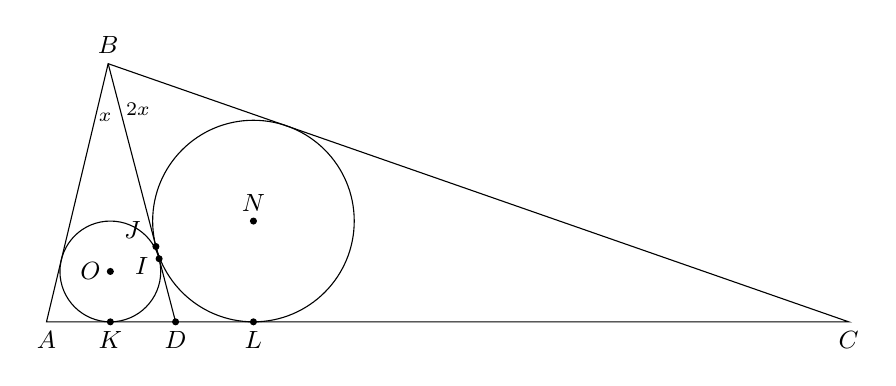
\begin{tikzpicture}[scale=0.16,font=\small]
\coordinate (D) at (0,0); \coordinate (B) at (-5.352,20.49); \coordinate (A) at (-10.247,0); \coordinate (C) at (53.43,0);
\coordinate (K) at (-5.179,0); \coordinate (L) at (6.179,0); \coordinate (O) at (-5.179,4); \coordinate (N) at (6.179,8); \coordinate (J) at (-1.561,5.978); \coordinate (I) at (-1.309,5.011);
\draw (A)--(B)--(C)--cycle; \draw (B)--(D); \draw (O) circle (4); \draw (N) circle (8);
\foreach \p in {D,K,L,O,N,I,J} \fill (\p) circle (8pt);
\node[above] at (B) {$B$}; \node[below] at (A) {$A$}; \node[below] at (C) {$C$}; \node[below] at (D) {$D$}; \node[below] at (K) {$K$}; \node[below] at (L) {$L$}; \node[left] at (O) {$O$}; \node[above] at (N) {$N$}; \node[left] at (-1.4,4.4) {$I$}; \node[left] at (-2.0,7.3) {$J$};
\node at (-5.6,16.2) {\scriptsize$x$}; \node at (-3.0,16.9) {\scriptsize$2x$};
\end{tikzpicture}}
\AB{$IJ$ kesma uzunligini toping.}{$BJ$ kesma uzunligini toping.}}
\QQ{44}{Öq kesimidan kesilgan yarim silindrdan eng katta hajmli parallelepiped öyib olingan. ($\pi=3$ deb oling.)
\qfig{\begin{tikzpicture}[scale=0.75,font=\small]
\draw (-1.5,0) arc (180:360:1.5); \draw (-1.5,0)--(1.5,0);
\fill[qfill] (-1.06,0) rectangle (1.06,-1.06); \draw (-1.06,0) rectangle (1.06,-1.06);
\draw (-1.5,0)--(0.5,2.4)--(3.5,2.4)--(1.5,0); \draw[dashed] (0.5,2.4) arc (180:240:1.5); \draw (3.5,2.4) arc (0:-62:1.5);
\draw (1.06,0)--(3.06,2.4); \draw (1.06,-1.06)--(3.06,1.34)--(3.06,2.4); \draw[dashed] (-1.06,-1.06)--(0.94,1.34)--(3.06,1.34); \draw (-1.06,0)--(0.94,2.4); \draw[dashed] (0.94,1.34)--(0.94,2.4);
\end{tikzpicture}}
\AB{Silindr asosi diametrining parallelepiped asosi diagonaliga nisbatini toping.}{Öyib olingan parallelepiped hajmining yarim silindr hajmiga nisbatini toping.}}
\QQ{45}{Silindrsimon idişga töla suv quyildi ($a$ — rasm). Söng idişni öqi tekislik bilan $30^\circ$ burçak hosil qiladigan qilib burişdi ($b$ — rasm) va yana joyiga qaytarişdi ($c$ — rasm). Agar $\dfrac H{2R}=\dfrac4{\sqrt3}$ bölsa:
\qfig{\begin{tikzpicture}[scale=0.55,font=\small]
\fill[qfill] (-0.9,0)--(-0.9,3.8) arc (180:360:0.9 and 0.2)--(0.9,0) arc (360:180:0.9 and 0.2);
\draw (0,3.8) ellipse (0.9 and 0.2); \draw (-0.9,0)--(-0.9,3.8); \draw (0.9,0)--(0.9,3.8); \draw (-0.9,0) arc (180:360:0.9 and 0.2); \draw[dashed] (0.9,0) arc (0:180:0.9 and 0.2);
\node[left] at (-0.9,1.9) {$H$}; \node[below] at (0,-0.5) {$a$ — rasm};
\begin{scope}[xshift=3cm]
\draw (-0.5,-0.2)--(5.2,-0.2);
\begin{scope}[shift={(1.3,-0.2)},rotate=30]
\fill[qfill] (0,0)--(0,1.8)--(0.66,1.8)--(3.8,0)--cycle;
\draw (0,0)--(3.8,0); \draw (0,1.8)--(3.8,1.8); \draw (3.8,0.9) ellipse (0.2 and 0.9); \draw (0,0.9) ellipse (0.2 and 0.9);
\end{scope}
\draw[thick] (1.3,-0.2)+(0:0.7) arc (0:30:0.7); \node at (2.35,0.05) {\scriptsize$30^\circ$};
\node[below] at (2.3,-0.5) {$b$ — rasm};
\end{scope}
\begin{scope}[xshift=10.5cm]
\fill[qfill] (-0.9,0)--(-0.9,2.4) arc (180:360:0.9 and 0.2)--(0.9,0) arc (360:180:0.9 and 0.2);
\draw (0,3.8) ellipse (0.9 and 0.2); \draw (0,2.4) ellipse (0.9 and 0.2); \draw (-0.9,0)--(-0.9,3.8); \draw (0.9,0)--(0.9,3.8); \draw (-0.9,0) arc (180:360:0.9 and 0.2); \draw[dashed] (0.9,0) arc (0:180:0.9 and 0.2);
\node[left] at (-0.9,1.2) {$h$}; \node[below] at (0,-0.5) {$c$ — rasm};
\end{scope}
\end{tikzpicture}}
\AB{$\dfrac hH$ ning qiymatini toping.}{Agar idişda töla suv $400$ litr bölsa, tökilgan suv neça litr?}}
\Javoblar{C B A D B A C C C C A C B D B C A B C D D C B C A B A D D A A C A D F}{%
\OK{36}{$2$}{$0$}\OK{37}{$7$}{$\dfrac{11\pi}6$}\OK{38}{$-12$}{$1$}\OK{39}{$3$}{$6$}\OK{40}{$3$}{$\dfrac83$}%
\OK{41}{$5\sqrt2$}{$10$}\OK{42}{$\dfrac{3\sqrt3-2}2$}{$2$}\OK{43}{$1$}{$15$}\OK{44}{$\dfrac{2\sqrt{10}}5$}{$\dfrac23$}\OK{45}{$\dfrac58$}{$150$}}
